%----------------------------------------------------------------------------
\chapter{\modeling}\label{chap:model}
%----------------------------------------------------------------------------
\section{Követelmény modellezés}
A modellezendő rendszerhez alapvetően EN 13452\cite{EN13452-1} szabvány első részében található funkcionális követelményeket vettem figyelembe.
Az \ref{fig:reqs} ábrán látható a követelmények modellje.
Ezen megjelenik a öt fő funkció, amit a rendszernek teljesítenie kell.

\begin{figure}
    \centering
    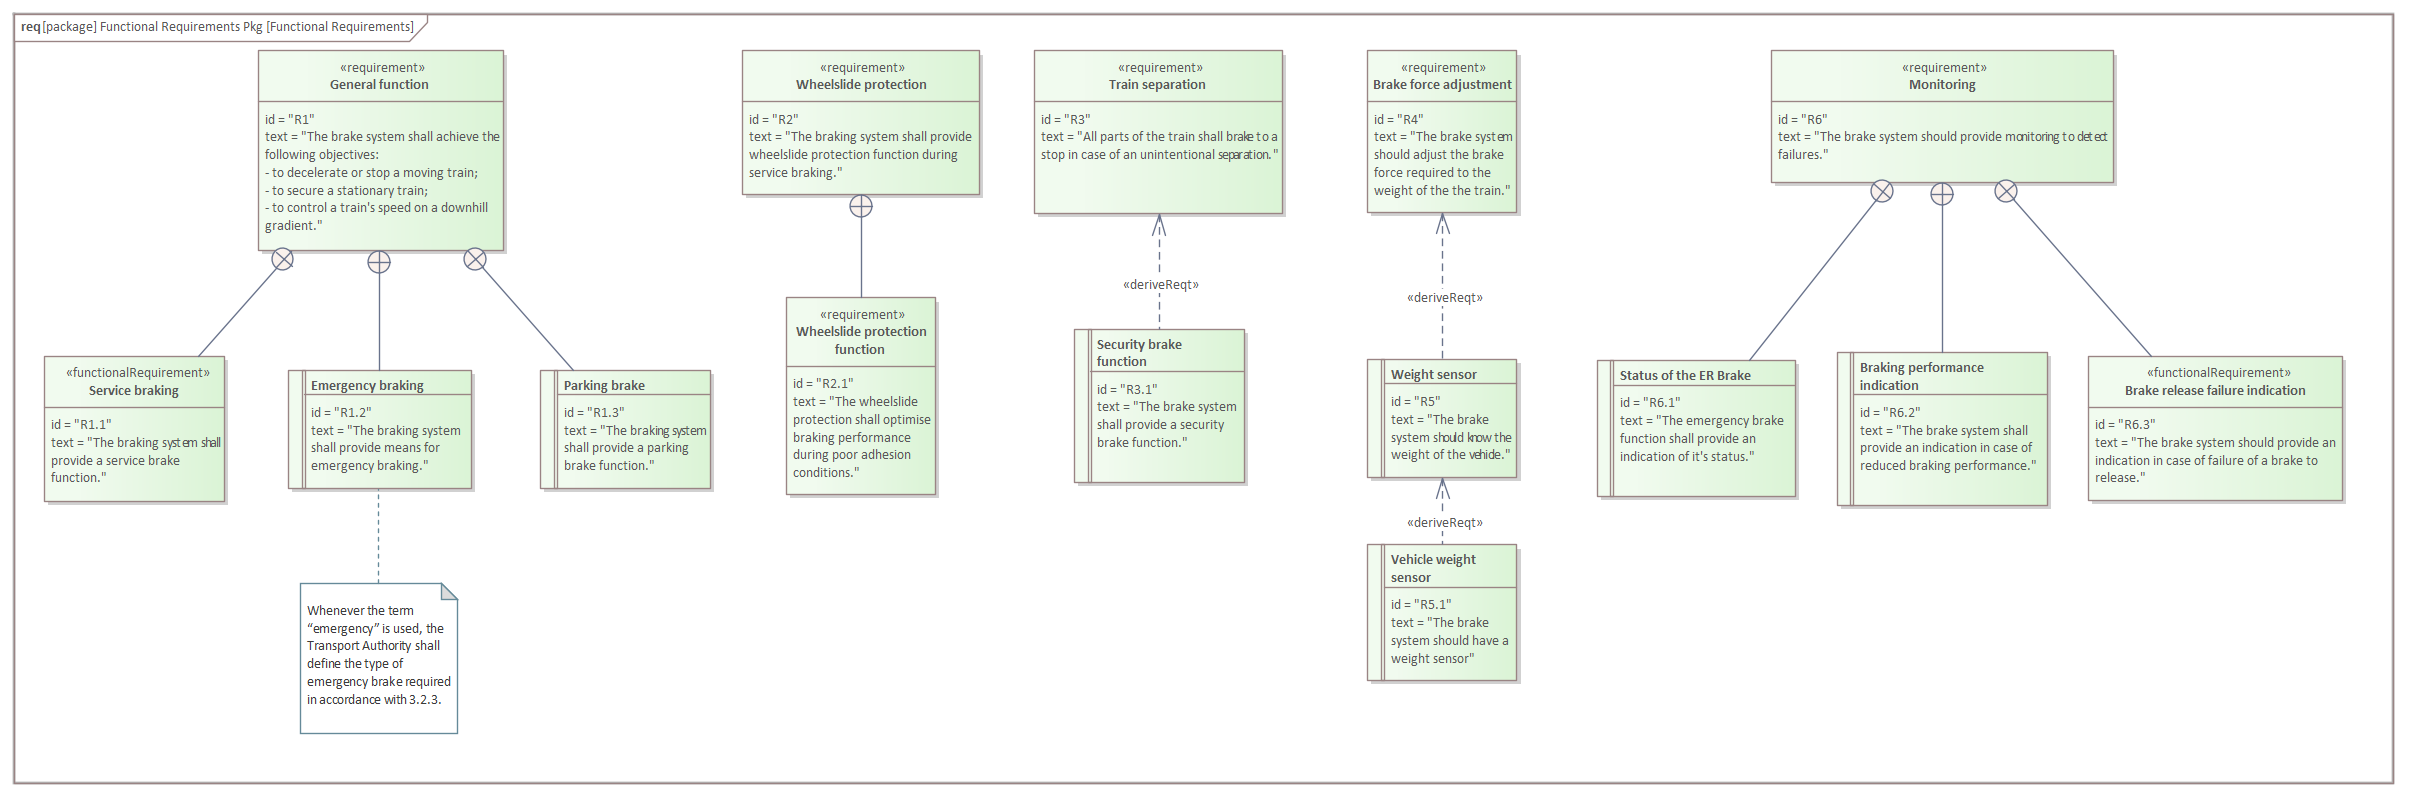
\includegraphics[height=200mm, keepaspectratio]{figures/Functional Requirements.png}
    \caption{A rendszer funkcionális követelményinek modellje SysML-ben.}
    \label{fig:reqs}
\end{figure}

\section{Funkcionális dekompozíció}
A \ref{fig:func_arch}. ábrán látható a funkcionális dekompozíciójának block definition diagram-ja.
Ezen látható, hogy a fékrendszer több elemet is támogat a \ref{sec:vjfr}. részben taglalt funkciók közül.
A rendszer a következő öt funkciókkal rendelkezik, ahogy az a \ref{fig:func_arch}. ábrán is látható: 
(1) üzemi fék (service brake), 
(2) vészfék (emergency brake), 
(3) biztonsági fék (security brake),
(4) parkoló fék (parking brake) és 
(5) kerékcsúszás gátlás (wheelslide protection).
Továbbá az ábrán az is látható, hogy a fékrendszer képes forgóvázra nehezedő súly által szabályozni a fékezési erőt.

\begin{figure}
    \footnotesize
    \centering
    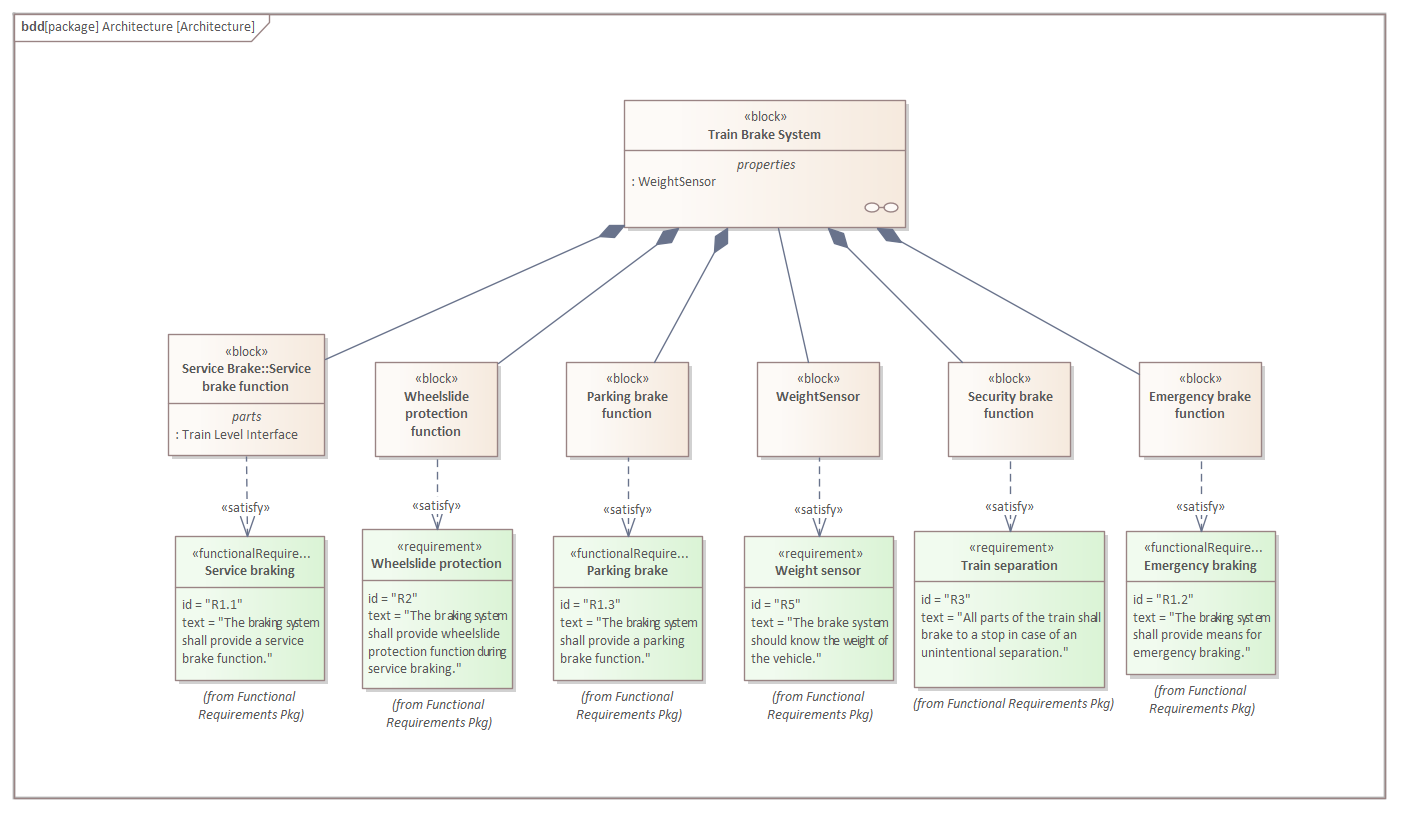
\includegraphics[width=150mm, keepaspectratio]{figures/Architecture.png}
    \caption{A tervezett fékrendszer funkcionális dekompozíciója}
    \label{fig:func_arch}
\end{figure}

A \ref{fig:func_arch_ibd}. ábrán látható a rendszer belső felépítése (IBD\footnote{internal block diagram}).
Az ábra tartalmazza és definiálja az alrendszerek kapcsolatát, továbbá leírja a rendszer külső csatlakozási pontjait portok által.
\begin{figure}
    \footnotesize
    \centering
    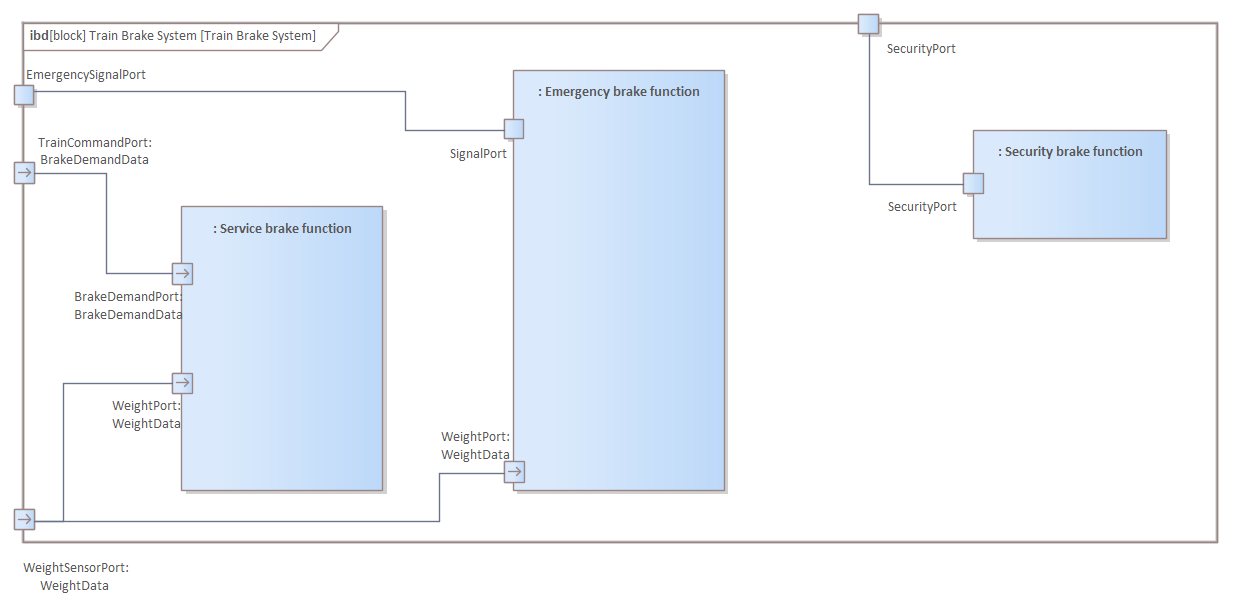
\includegraphics[width=150mm, keepaspectratio]{figures/Architecture_ibd.png}
    \caption{A fékrendszer belső felépítése}
    \label{fig:func_arch_ibd}
\end{figure}

\subsection{Üzemi fék}
Az dekompozíciós folyamatot az üzemi fék alrendszeren folytatva a \ref{fig:service_brake_bdd}. ábra mutatja az üzemi fék funkcionális felbontását/BDD\footnote{Block Definition Diagram}-jét.
Az ábrán látható, hogy ez egy vezérlő funkció ezért megjelenik a vezérlő-rendszer-visszacsatoló hármas a modellben.
Továbbá az is látszik, hogy a vezérlő funkció egy összetett eleme az alegységnek.

\begin{figure}
    \footnotesize
    \centering
    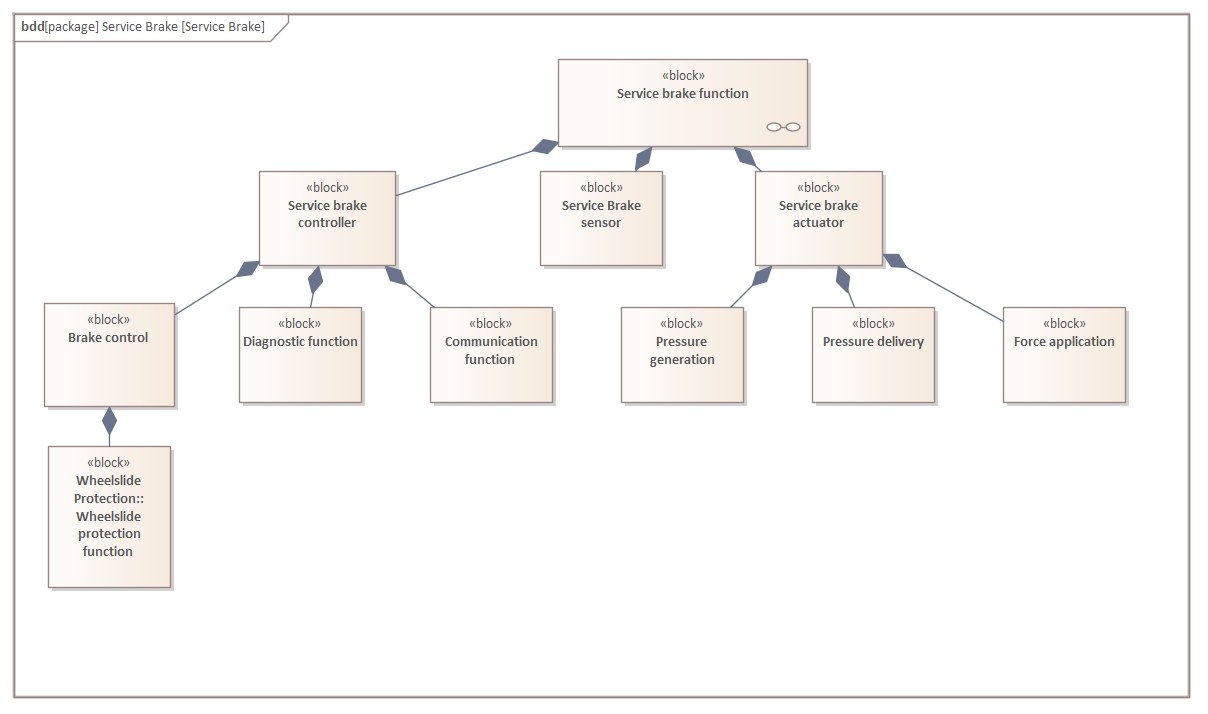
\includegraphics[width=150mm, keepaspectratio]{figures/Service_Brake_bdd.png}
    \caption{Üzemi fék blokk definition diagramm-ja.}
    \label{fig:service_brake_bdd}
\end{figure}

\section{Platform modellezés}
Ebben a részben a fentebb elkészített funkciónális modellhez tartozó platform modellt fogom bemutatni.
SysML-ben platform modelleket használunk arra a célra, hogy a megtervezett funkciókat ténylegesen hardver/softver elemekhez allokáljuk.
Ezek a modellek már a valódi fizikai alkatrészeket, illetve ezek kapcsolátát reprezentálják.
Ebben a fázisban általában Bottom-up tervezési elvet használnak, hiszen ez a folyamat nagyon hasonlít arra, amikor egy nyomtatott áramkört tervezünk és inkább alkatrészkönyvtárakból válogatnak a mérnökök.

\subsection{Aktuátorok}
A \ref{fig:act}. ábrán láthatók a fékrendszer azon aktuátorai, melyek részt vesznek a fékezés folyamatában.
Az ábrán látható NC\footnote{Normally Closed} jelölés megjelenik mind a vezérlő szelepnél (valve), mind a fékollónál (brake caliper).
Az előbbi esetében ez azt jelenti, hogy ameddig nem kap megfelelő feszültséget a bemeneti csatlakozóján addig nyitva tartja a hidraulikus folyadék útját a gyűjtőtartály felé, ezzel csökkentve/elengedve a hidraulikus rendszerben lévő nyomást.
A fékolló esetében pedig azt jelenti, hogy egy olyan mechanikai megoldást alkalmaz, amely rugós előfeszítéssel fékezi a hozzá tartozó féktárcsát.
Az eszközt hidraulikus nyomás segítségével lehet leoldani/lazítani a féktárcsáról, ezáltal a rendszer örökölten képes támogatni a parkoló fék funkciót.

\begin{figure}
    \centering
    \footnotesize
    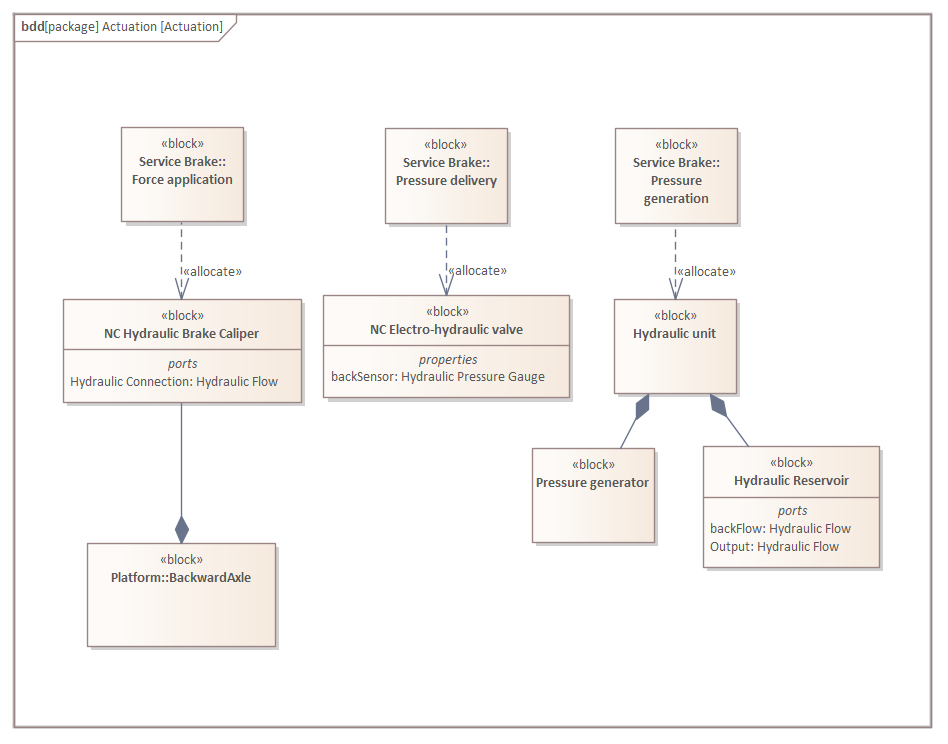
\includegraphics[width=150mm, keepaspectratio]{figures/Platform_Actuation_bdd.png}
    \caption{A fékrendszer aktuátorainak platform modellje.}
    \label{fig:act}
\end{figure}

Ezen alkatrészek segítségével már az összes olyan funkciót meg lehet valósítani, ami a kívánt fékezési erőt képes átadni az adott tengelyre.


\subsection{Elektronikai vezérlő}
Az elektro-hidraulikus fékrendszer elengedhetetlen rész a vezérlő elektronika.
Ez a részegység felelős a hidraulikus rendszer irányításáért, ellenőrzéséért és a hibajelzésért.

Általában ez az egység képezi a forgóvázon elhelyezett fékrendszer legösszetettebb részét.
Továbbá itt található meg a legtöbb biztonság-kritikus funkció is.
A \ref{fig:control_elect}. ábrán látható a vezérlőelektronika blokkdefiníciós diagrammja.

Az ábrán látható, hogy a rendszer nem annyira összetett, mint a valóságban, de szerepelnek rajta olyan elemek, melyek megjelennek egy tényleges projektben.
Ezek például az analóg-digitális és digitális-analóg átalakítók, beágyazott vezérlő processzot valósidejű operációs rendszert futtatva, illetve a hozzá tartozó memória illetve kommunikációs modulok.

\begin{figure}
    \footnotesize
    \centering
    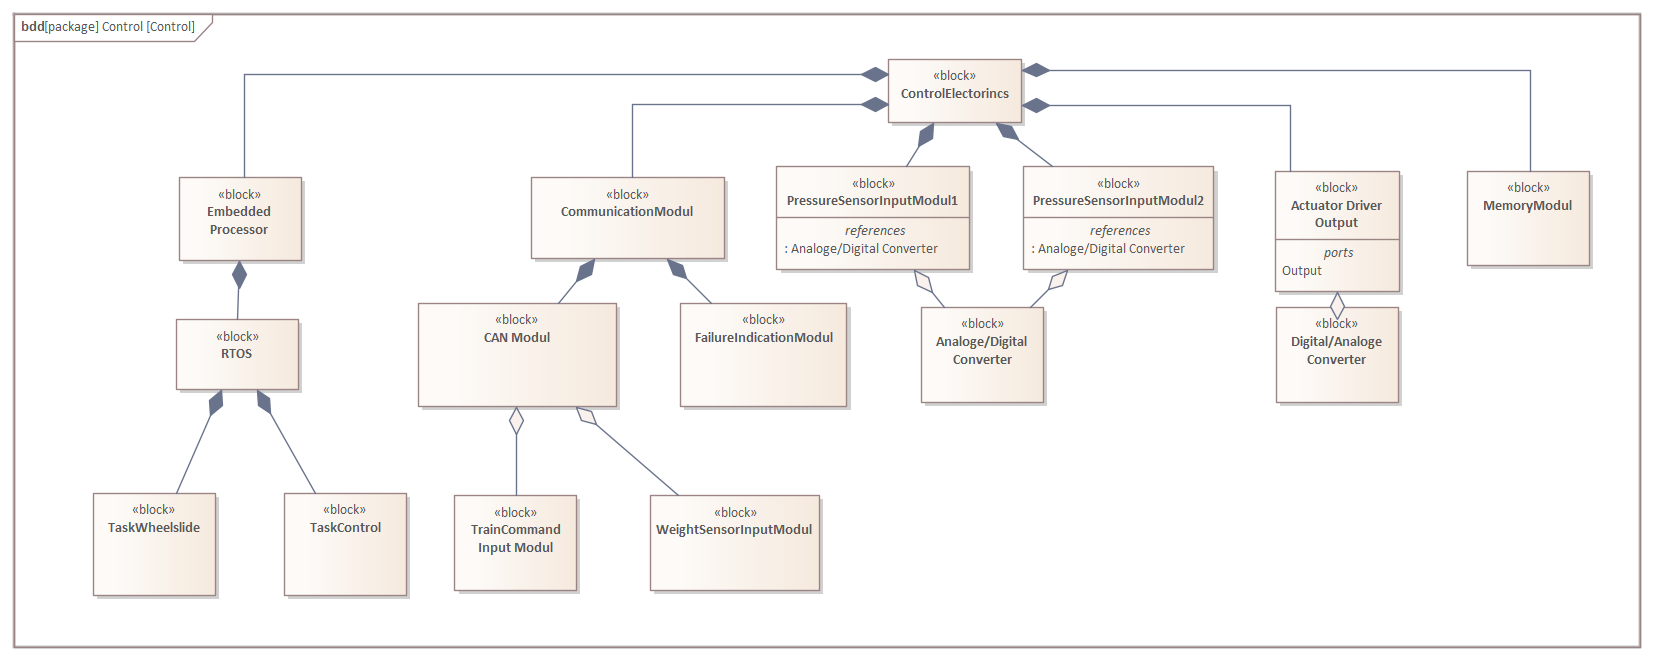
\includegraphics[width=150mm, keepaspectratio]{figures/Platform_Control_bdd.png}
    \caption{A vezérlő elektronika platform modellje bdd-n bemutatva.}
    \label{fig:control_elect}
\end{figure}

\subsection{Platform architektúra modell}
Végezetül elkészítettem a fentebb említett kisebb egységek összekapcsolásával/kombinálásával az egy forgóvázon (bogie-n) elhelyezhető, kompakt fékrendszert.
Mint az a \ref{fig:plat_arch}. ábrán látható, a fékrendszer két független fékkörrel rendelkezik, amely képes a forgóvázon lévő mind a két tengelyt fékezni.

Ezen redundancia alkalmazásával a rendszer képes elegendő fékerőt generálni, még ha esetlegesen az egyik fékkör meghibásodna.

\begin{figure}
    \footnotesize
    \centering
    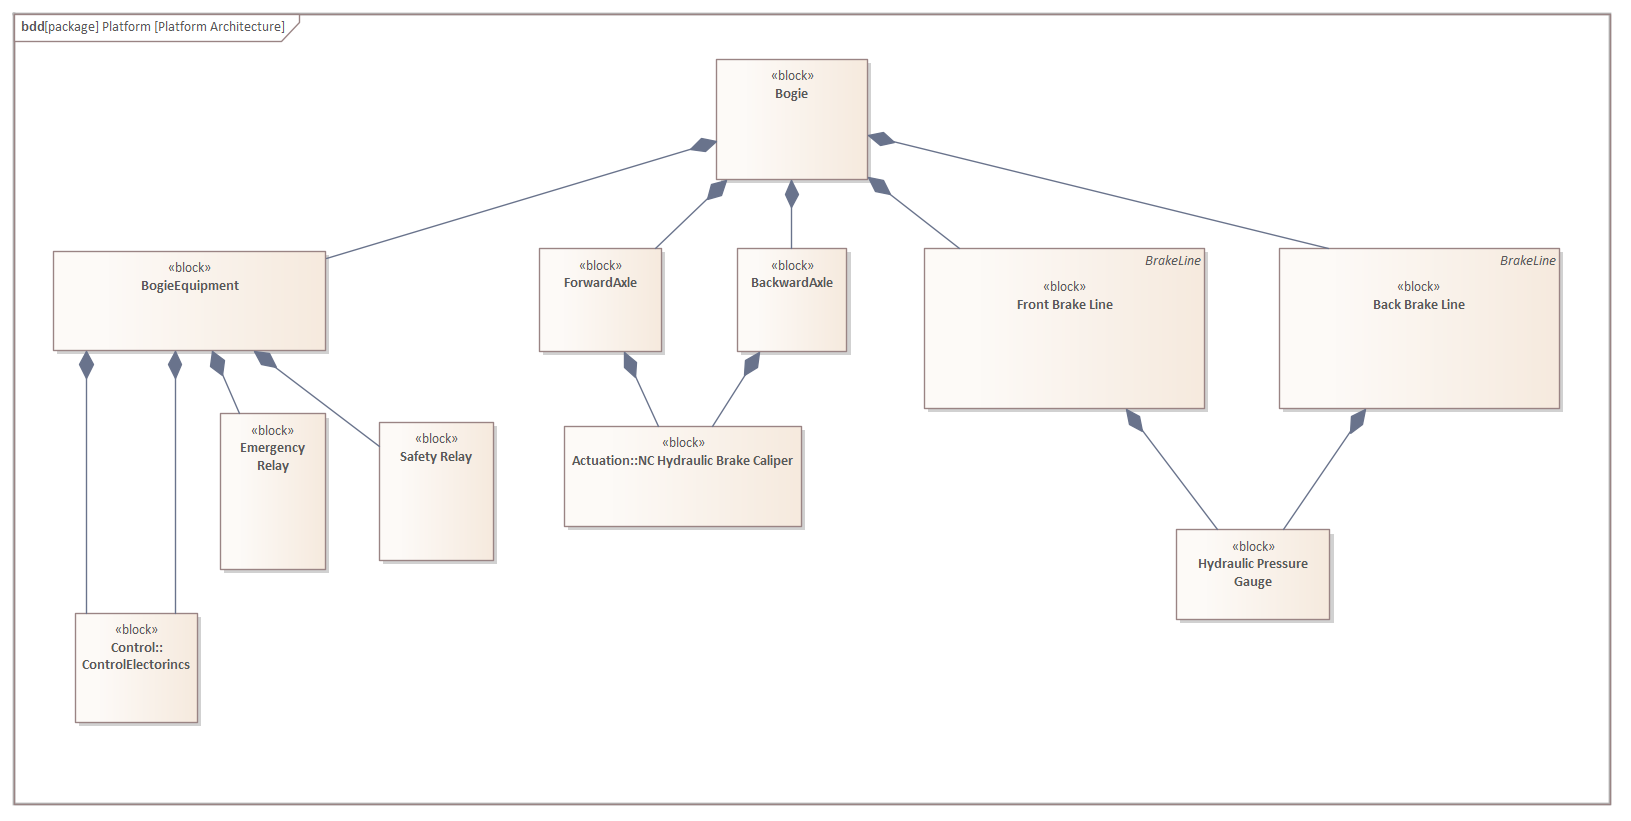
\includegraphics[width=150mm, keepaspectratio]{figures/Platform_Architecture_bdd.png}
    \caption{A fékrendszer platform modelljének architektúrája bdd-n ábrázolva.}
    \label{fig:plat_arch}
\end{figure}

A \ref{fig:plat_ibd}. ábra szemlélteti a rendszer összeköttetéseit, az alkatrészek kapcsolatát.
Ezen már megjelenik a teljes mértékben összekapcsolt hidraulikus rendszer a két függetlenül vezérelt hidraulikus körrel, illetve az úgynevezett BogieEquipment (BE), ami az iparágban a forgóvázra felszerelhető egységet jelenti.

A BE tartalmazza általában a vezérlő elektronikát és a hozzá tartozó csatlakozási pontokat is.
Ezt a fentebb említett ábra is remekül szemlélteti, hiszen ebben az egységben helyezkedik el mind a két vezérlő elem, illetve a biztonsági és vészfék irányíttó kapcsoló is.

\begin{figure}
    \footnotesize
    \centering
    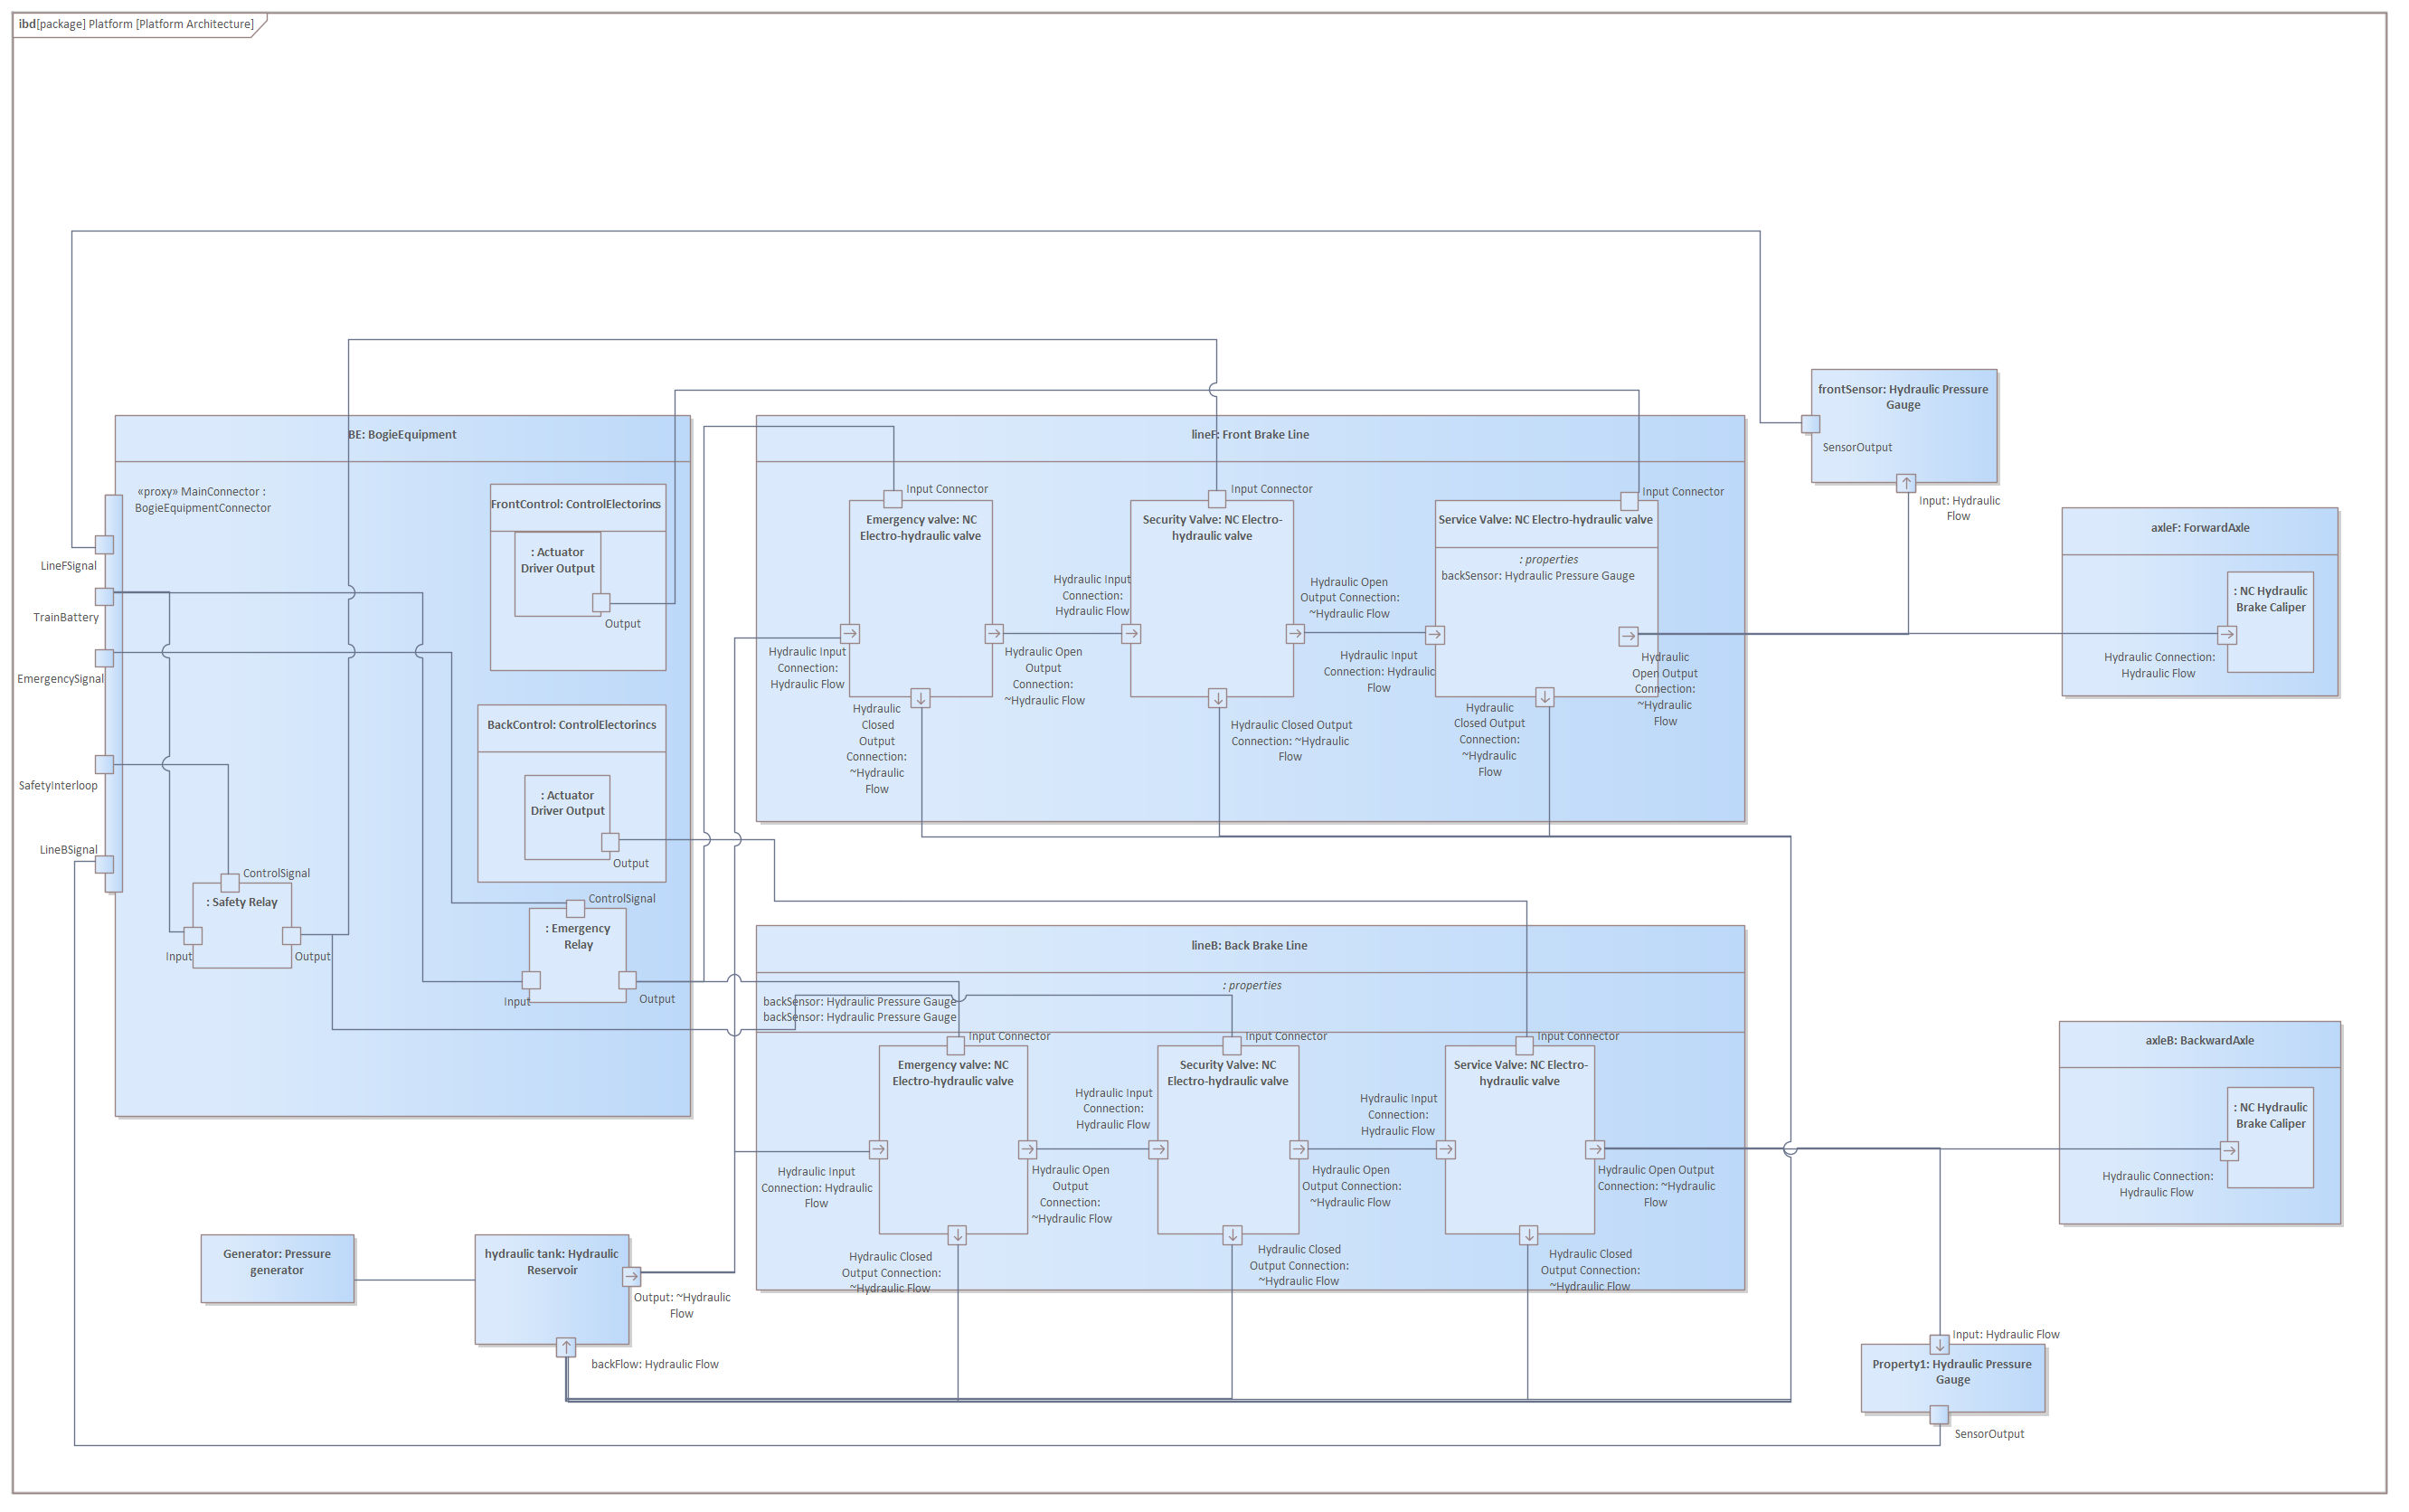
\includegraphics[width=150mm,keepaspectratio]{figures/Platform_Architecture_ibd.png}
    \caption{A fékrendszer fizikai összeköttetései, alkatrészeinek kapcsolata ibd-n ábrázolva.}
    \label{fig:plat_ibd}
\end{figure}